\documentclass[10pt]{article}
\usepackage[pdftex]{graphicx, color}
\usepackage{listings,proof}
\usepackage{minted}
\usepackage{tikz}
\usepackage{hyperref}
\usetikzlibrary{automata,positioning}

\headheight 8pt \headsep 20pt \footskip 30pt
\textheight 9in \textwidth 6.5in
\oddsidemargin 0in \evensidemargin 0in
\topmargin -.35in
\lstset{
  basicstyle=\ttfamily,
  mathescape
}
\lstset{basicstyle=\small\ttfamily,breaklines=true}
\newcommand {\pts}[1]{{\bf #1 pts}}
\newcommand{\ttmath}[1]{$\mathtt{#1}$}
\newcommand{\ossimple}[6]{#1,#2,#3\vdash #4 : #5,#6}
\newcommand{\osrule}[8]{\frac{#7}{\ossimple{#1}{#2}{#3}{#4}{#5}{#6}}\eqno
  \mbox{#8}}
\newcommand{\infertext}[2]{\infer{{\textrm{#1}}}{#2}}

\begin{document}
\begin{center}
  \Large CS131 Compilers: Writing Assignment 4\\
  Due Tue, May 31, 2022 at 23:59pm
\end{center}

\begin{center}
  %% Change this:
  \LARGE Tian Haoyuan - 2020533013
\end{center}

This assignment asks you to prepare written answers to questions on
semantic analysis. Each of the questions has a short answer. You
may discuss this assignment with other students and work on the problems
together. However, your write-up should be your own individual work.
and you should indicate in your submission who you worked with, if applicable.
Written assignments are turned in at the start of lecture.
You should use the Latex template provided at the course web site to write your solution.

\begin{center}
  %% Change this:
  I worked with: nobody
\end{center}

\begin{enumerate}
  \item \textbf{Activation Records. } For each of the variable $a, b, c, d, e$ in this C program, say whether
        the variable should be kept in memory or a register, and why.
        \begin{verbatim}
        int f(int a, int b)
        { int c[3], d, e;
          d = a+1;
          e=g(c,&b);
          return e+c[1]+b;
        }
        \end{verbatim}
        \textcolor{blue}{
          % a,b should be kept in registers, and c,e,d should be kept in memory.\\
          a,b,c,d,e should all be kept in memory. \\Since a,b are formal parameters that is local to the procedure f(). These are pass by value, so a,b get the copy of real parameters (kept in register), and they are kept in stack.\\
          c,d,e are local variables of the procedure f(). They are kept in stack.
        }
  \item \textbf{Activation Records. } In the C code to compute Fibonacci numbers recursively. Suppose that the
        activation record for f includes the following elements
        in order: (return value, argument $n$, local $s$, local $t$); there will normally be
        other elements in the activation record as well. The questions below assume
        that the initial call is f (5).
        \begin{verbatim}
    int f(int n) {
        int t, s;
        if (n < 2) return 1;
        s = f(n-1);
        t = f(n-2);
        return s+t;
    }
    \end{verbatim}
        \begin{enumerate}
          \item Show the complete activation tree.
                \textcolor{blue}{\\
                  \begin{tikzpicture}    [
                      level distance = 2.5em,
                      level 1/.style={sibling distance=6cm},
                      level 2/.style={sibling distance=3cm},
                      level 3/.style={sibling distance=2cm}
                    ]
                    \node(root){f(5)}
                    child{node{f(4)}
                        child{node{f(3)}
                            child{node{f(2)}
                                child{node{f(1)}
                                  }
                                child{node{f(0)}
                                  }
                              }
                            child{node{f(1)}
                              }
                          }
                        child{node{f(2)}
                            child{node{f(1)}
                              }
                            child{node{f(0)}
                              }
                          }
                      }
                    child{node{f(3)}
                        child{node{f(2)}
                            child{node{f(1)}
                              }
                            child{node{f(0)}
                              }
                          }
                        child{node{f(1)}
                          }
                      };
                  \end{tikzpicture}
                }
          \item What does the stack and its activation records look like the first time f(1) is about to return?
                \textcolor{blue}{\\
                  Let the stack bottom be the top of the table.\\
                  \begin{tabular}{|c|}
                    \hline
                    \hline
                    \\
                    \hline
                    $f(5)$retval   \\
                    \hline
                    $n=5$          \\
                    \hline
                    control link   \\
                    \hline
                    access link    \\
                    \hline
                    $s=f(4)$       \\
                    \hline
                    $t=f(3)$       \\
                    \hline
                    $f(4)$retval   \\
                    \hline
                    $n=4$          \\
                    \hline
                    control link   \\
                    \hline
                    access link    \\
                    \hline
                    $s=f(3)$       \\
                    \hline
                    $t=f(2)$       \\
                    \hline
                    $f(3)$retval   \\
                    \hline
                    $n=3$          \\
                    \hline
                    control link   \\
                    \hline
                    access link    \\
                    \hline
                    $s=f(2)$       \\
                    \hline
                    $t=f(1)$       \\
                    \hline
                    $f(2)$retval   \\
                    \hline
                    $n=2$          \\
                    \hline
                    control link   \\
                    \hline
                    access link    \\
                    \hline
                    $s=f(1)$       \\
                    \hline
                    $t=f(0)$       \\
                    \hline
                    $f(1)$retval=1 \\
                    \hline
                    $n=1$          \\
                    \hline
                    control link   \\
                    \hline
                    access link    \\
                    \hline
                    \\
                  \end{tabular}
                }
          \item What does the stack and its activation records look like the fifth time f(1) is about to return?
                \textcolor{blue}{\\
                  Let the stack bottom be the top of the table.\\
                  \begin{tabular}{|c|}
                    \hline
                    \hline
                    \\
                    \hline
                    $f(5)$retval   \\
                    \hline
                    $n=5$          \\
                    \hline
                    control link   \\
                    \hline
                    access link    \\
                    \hline
                    $s=5$          \\
                    \hline
                    $t=f(3)$       \\
                    \hline
                    $f(3)$retval   \\
                    \hline
                    $n=3$          \\
                    \hline
                    control link   \\
                    \hline
                    access link    \\
                    \hline
                    $s=2$          \\
                    \hline
                    $t=f(1)$       \\
                    \hline
                    $f(1)$retval=1 \\
                    \hline
                    $n=1$          \\
                    \hline
                    control link   \\
                    \hline
                    access link    \\
                    \hline
                    \\
                  \end{tabular}
                }
        \end{enumerate}
  \item \textbf{Code Generation. } Suppose a basic block is formed from the C assignment statements
        \begin{verbatim}
        x = a + b + c + d + e + f;
        y = a + c + e;
    \end{verbatim}
        \begin{enumerate}
          \item Give the three-address statements (only one addition per statement) for this block.\\
                \textcolor{blue}{
                  $t_1=a+b\\
                    t_2=t_1+c\\
                    t_3=t_2+d\\
                    t_4=t_3+e\\
                    t_5=t_4+f\\
                    x=t_5\\
                    t_6=a+c\\
                    t_7=t_6+e\\
                    y=t_7$
                }
          \item Use the associative and commutative laws to modify the block to use the fewest possible number of
                instructions, assuming both x and y are live on exit from the block.
                \textcolor{blue}{\\
                  $t_1=a+c\\
                    t_2=t_1+e\\
                    y=t_7\\
                    t_3=t_7+b\\
                    t_4=t_3+d\\
                    t_5=t_4+f\\
                    x=t_5\\
                  $
                }
        \end{enumerate}
  \item \textbf{Run-time environment. } Here is a sketch of two C functions $f$ and $g$:
        \begin{verbatim}
        int f(int x){int i;...return i+1;...}
        int g(int y) {int j;...f(j+1). ..}
    \end{verbatim}
        That is, function $g$ calls $f$ . Draw the top of the stack, starting with the activation record for $g$,
        after $g$ calls $f$ , and $f$ is about to return. You can consider
        only return values, parameters, control links, and space for local variables; you
        do not have to consider stored state or temporary or local values not shown in
        the code sketch. Answer the following questions:
        \textcolor{blue}{\\
          Let the stack bottom be the top of the table.\\
          \begin{tabular}{|c|}
            \hline
            \hline
            (*)                        \\
            \hline
            g() retval                 \\
            \hline
            int y                      \\
            \hline
            (**) control link to (*)   \\
            \hline
            int j                      \\
            \hline
            f() retval                 \\
            \hline
            int x                      \\
            \hline
            (***) control link to (**) \\
            \hline
            int i                      \\
            \hline
            \\
          \end{tabular}
        }
        \begin{enumerate}
          \item Which function creates the space on the stack for each element?
                \textcolor{blue}{\\
                  The caller of g() creates the space of g() retval, int y, control link to (*).\\
                  g() creates the space of int j, f() retval, int x, control link to (**).\\
                  f() creates the space of int i.
                }
          \item Which function writes the value of each element?
                \textcolor{blue}{\\
                  The caller of g() writes the value of control link to(*).\\
                  g() writes the value of g() retval, int y, control link to(**), int j.\\
                  f() writes the value of f() retval, int x, int i.
                }
          \item To which activation record does the element belong?
                \textcolor{blue}{\\
                  int y and int j belong to the activation record of g().\\
                  int x and int i belong to the activation record of f().
                }
        \end{enumerate}
  \item \textbf{Code Optimization} Consider the following basic block, in which all variables are integers, and
        ** denotes exponentiation.
        \begin{verbatim}
        a := b + c
        z := a ** 2
        x := 0 * b
        y := b + c
        w := y * y
        u := x + 3
        v := u + w
    \end{verbatim}
        Assume that the only variables that are live at the exit of this block are v and z. In order, apply the
        following optimizations to this basic block. Show the result of each transformation.
        \begin{enumerate}
          \item algebraic simplification
                \begin{verbatim}
                    a := b + c
                    z := a * a
                    x := 0
                    y := b + c
                    w := y * y
                    u := x + 3
                    v := u + w
                  
    \end{verbatim}
          \item common sub-expression elimination
                \begin{verbatim}
                    a := b + c
                    z := a * a
                    x := 0
                    y := a
                    w := y * y
                    u := x + 3
                    v := u + w
    \end{verbatim}
          \item copy propagation
                \begin{verbatim}
                    a := b + c
                    z := a * a
                    x := 0
                    y := a
                    w := a * a
                    u := 0 + 3
                    v := u + w
    \end{verbatim}
          \item constant folding
                \begin{verbatim}
                    a := b + c
                    z := a * a
                    x := 0
                    y := a
                    w := a * a
                    u := 3
                    v := u + w
    \end{verbatim}
          \item dead code elimination
                \begin{verbatim}
                    a := b + c
                    z := a * a
                    w := a * a
                    u := 3
                    v := u + w
    \end{verbatim}
        \end{enumerate}
  \item \textbf{Code Optimization} Consider the following C code
        \begin{minted}[mathescape,linenos]{c}
int d[10][10];
for(int k = 0; k < 10; k++)
for(int i = 0; i < 10; i++)
for(int j = 0; j < 10; j++)
if(d[i][j] > d[i][k] + d[k][j])
d[i][j] = d[i][k] + d[k][j];
    \end{minted}
        \begin{enumerate}
          \item Gives the three-address code for the innermost j loop of the layer.
                \begin{verbatim}
  j = 0
  t1 = j
L1:
  if t1 >= 10 goto L2
  t2 = i * 10
  t3 = t2 + j
  t4 = t3 * 4
  t5 = d[t4]      // t5 is d[i][j]
  t6 = i * 10
  t7 = t6 + k
  t8 = t7 * 4
  t9 = d[t8]      // t9 is d[i][k]
  t10 = k * 10
  t11 = t10 + j
  t12 = t11 * 4
  t13 = d[t12]    // t13 is d[k][j]
  t14 = t9 + t13
  if t5 <= t14 goto L3
  t15 = i * 10
  t16 = t15 + k
  t17 = t16 * 4
  t18 = d[t17]      // t18 is d[i][k]
  t19 = k * 10
  t20 = t19 + j
  t21 = t20 * 4
  t22 = d[t21]      // t22 is d[k][j]
  t23 = t18 + t22
  t24 = i * 10
  t25 = t24 + j
  t26 = t25 * 4
  d[t26] = t22
L3:
  t27 = j + 1
  j = t27 
  goto L1
L2:
\end{verbatim}
          \item The loop optimization is performed directly on the C source program (including loop-invariant
                extraction, Inductive variables strength weakening, etc.).
                \begin{minted}[mathescape,linenos]{c}
int d[10][10];
for(int k = 0; k < 10; k++)
{
    int *temp_k = d[k];
    for(int i = 0; i < 10; i++)
    {
        int temp_ik = d[i][k];
        for(int j = 0; j < 10; j++)
        {
            int temp_sum = temp_ik + temp_k[j];
            if(d[i][j] > temp_sum)
                d[i][j] = temp_sum;
        }
    }
}
                      \end{minted}
        \end{enumerate}
  \item \textbf{Register Allocation. } Consider the following program, annotated with live variable information:
        \begin{verbatim}
        // live: {v, x}
        u = v + 1
        // live: {u, v, x}
        w = u - v
        // live: {u, w, x}
        x = x + w
        // live: {u, w, x}
        y = u - w
        // live: {x, y}
        z = x + y
        // live {z}
    \end{verbatim}
        \begin{enumerate}
          \item Draw the interference graph for the program.
                \textcolor{blue}{\\
                  \begin{tikzpicture}[
                      auto,
                      node distance = 3cm, % distance between nodes
                      ,scale=.8,auto=left]
                    \node (v) at (2,0)		{v};
                    \node (u) at (4,0)  {u};
                    \node (w) at (0,-1.5) 	{w};
                    \node (x) at (2,-3) 	{x};
                    \node (y) at (4,-3) 	{y};
                    \node (z) at (6,-1.5) 	{z};
                    \draw (v)--(u);
                    \draw (v)--(x);
                    \draw (u)--(x);
                    \draw (w)--(x);
                    \draw (w)--(u);
                    \draw (x)--(y);
                  \end{tikzpicture}
                }
          \item What is the smallest number of colors that can be used to color the graph without spilling?
                Explain why no smaller number of colors will be enough.
                \textcolor{blue}{\\
                  The smallest number of colors is 3.\\
                  As the largest complete graph in this graph is K3, i.e. the subgraph uvx and edges between them, also the subgraph wux and edges between them. So clearly uvx are connected to each other, they must all use different colors, so the number of colors can't be less then 3.
                }
          \item Suppose you have machine registers $r1$, $r2$, and $r3$. Write an allocation of variables to
                registers such that no two adjacent variables have the same register, spilling if necessary.
                \textcolor{blue}{\\
                  Let the stack bottom be the bottom of the table.\\
                  Construct the stack by each time push a node that is the least connected into the stack, and deleting it's related edges, until all nodes are in the stack.\\
                  \begin{tabular}{|c|}
                    \\
                    \hline
                    u \\
                    \hline
                    x \\
                    \hline
                    w \\
                    \hline
                    v \\
                    \hline
                    y \\
                    \hline
                    z \\
                    \hline
                    \hline
                  \end{tabular}\\
                  Then from the top of the stack, distribute a register that would not cause error to the node, and pop the stack, until the stack is empty.\\
                  \begin{tabular}{|c|c}
                    \\
                    \hline
                    u & r1 \\
                    \hline
                    x & r2 \\
                    \hline
                    w & r3 \\
                    \hline
                    v & r3 \\
                    \hline
                    y & r1 \\
                    \hline
                    z & r1 \\
                    \hline
                    \hline
                  \end{tabular}
                  \\
                  So, an allocation can be $u:r1,x:r2,w:r3,v:r3,y:r1,z:r1$.
                }
        \end{enumerate}
  \item (10 pts) Consider the following RISCV assembly code program.  Using the
        stack-machine based code generation rules from lecture, what source program produces this
        code?
        \begin{verbatim}
f:
  addi    sp,sp,-48
  sw      s0,44(sp)
  addi    s0,sp,48
  sw      a0,-36(s0)
  sw      a1,-40(s0)
  sw      zero,-20(s0)
  sw      zero,-24(s0)
  j       .L2
.L3:
  lw      a5,-24(s0)
  slli    a5,a5,2
  lw      a4,-36(s0)
  add     a5,a4,a5
  lw      a5,0(a5)
  lw      a4,-20(s0)
  add     a5,a4,a5
  sw      a5,-20(s0)
  lw      a5,-24(s0)
  addi    a5,a5,1
  sw      a5,-24(s0)
.L2:
  lw      a4,-24(s0)
  lw      a5,-40(s0)
  blt     a4,a5,.L3
  lw      a5,-20(s0)
  mv      a0,a5
  lw      s0,44(sp)
  addi    sp,sp,48
  jr      ra
\end{verbatim}
        \begin{verbatim}
int f(int *arr, int n)
{
    int sum;
    int i;
    for (i = 0; i < n; ++i)
    {
        sum += arr[i];
    }
    return sum;
}
  \end{verbatim}
  \item (10*3=30 pts) Consider the following Cool program:
        \begin{verbatim}
class C {
  x : C; y : C;
  setx(newx : C) : C { x <- newx };
  sety(newy : C) : C { y <- newy };
  setxy(newx : C, newy :C) : SELF_TYPE {{ x <- newx; y <- newy; self; }};
};

class Main {
  x:C;
  main() : Object {
    let a : C <- new C, b :C <- new C, c : C<- new C, d : C <- new C,
    e : C <- new C, f :C <- new C, g : C <- new C, h : C <- new C in {
      f.sety(a), a.setxy(e, c); b.setx(d); g.setxy(d,f); c.sety(h); h.setxy(e, g); x <- c;
    }
  };
};
\end{verbatim}
        \begin{enumerate}
          \item (10 pts) Draw the heap at the end of execution of the above program, identifying objects by the variable
                names to which they are bound in the let expression. Assume that the root is the Main object created at the start
                of the program, and this object is not in the heap (note that Main is pointing to c).
                %
                \textcolor{blue}{\\
                  \begin{center}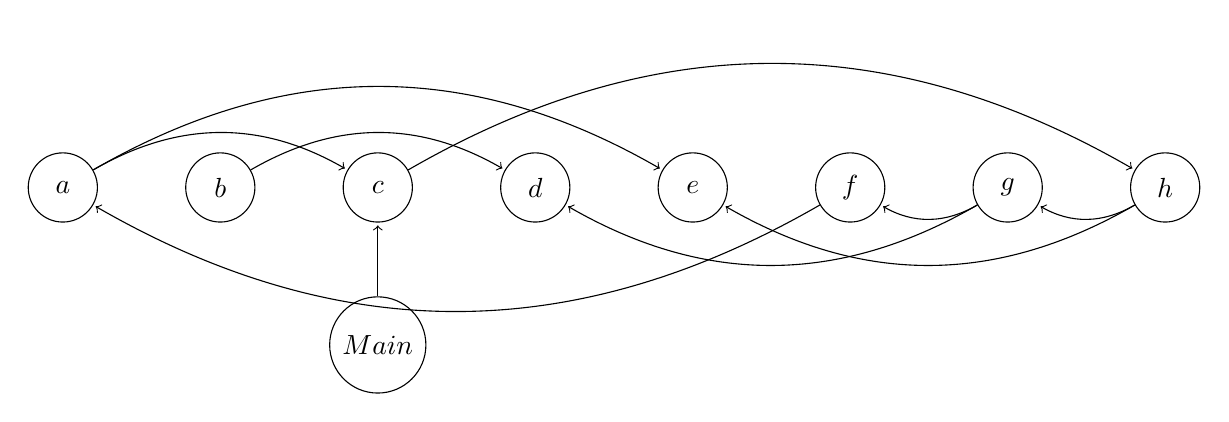
\begin{tikzpicture}[shorten >=1pt,node distance=2cm,on grid,auto]
                      \node[state] 			(a) 					{$a$};
                      \node[state] 			(b) 	[right=of a]	{$b$};
                      \node[state]			(c) 	[right=of b] 	{$c$};
                      \node[state] 			(d) 	[right=of c] 	{$d$};
                      \node[state] 			(e) 	[right=of d] 	{$e$};
                      \node[state] 			(f) 	[right=of e]	{$f$};
                      \node[state] 			(g) 	[right=of f]	{$g$};
                      \node[state] 			(h) 	[right=of g]	{$h$};
                      \node[state] 			(main) 	[below=of c]	{$Main$};
                      \path[->]
                      (a) 	edge	[bend left]		node 	{} 		(e)
                      edge	[bend left] 	node 	{} 		(c)
                      (b)		edge	[bend left] 	node 	{} 		(d)
                      (c)		edge	[bend left] 	node 	{} 		(h)
                      (f) 	edge	[bend left] 	node 	{} 		(a)
                      (g) 	edge	[bend left] 	node 	{} 		(f)
                      edge	[bend left] 	node 	{} 		(d)
                      (h) 	edge 	[bend left] 	node 	{} 		(e)
                      edge 	[bend left] 	node 	{} 		(g)
                      (main) edge [ ] node {} (c);
                    \end{tikzpicture}\end{center}
                }
          \item (10 pts) For each of the garbage collection algorithms discussed in class (Mark and Sweep, Copy Collector,
                Reference Counting), show the heap after garbage collection.
                %
                \textcolor{blue}{\\
                  Mark and Sweep
                  \begin{center}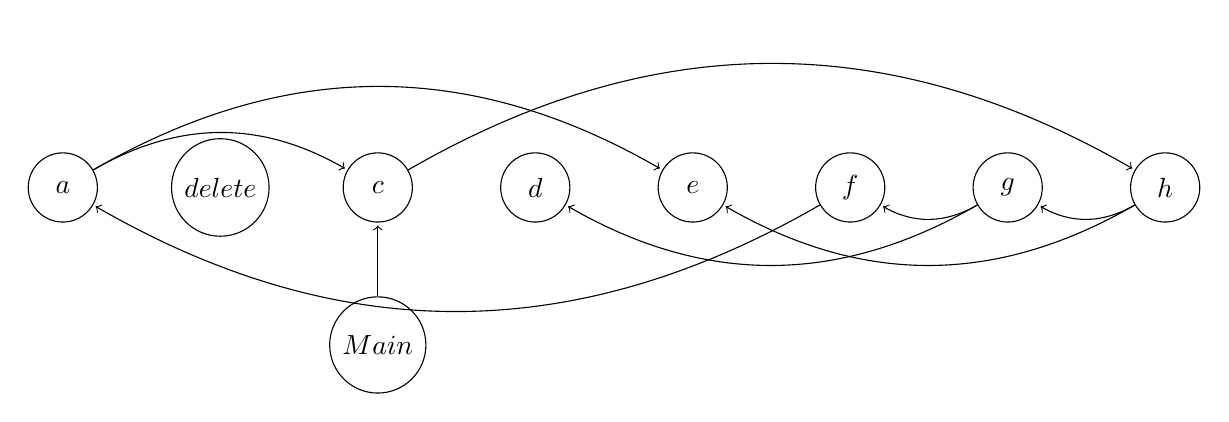
\begin{tikzpicture}[shorten >=1pt,node distance=2cm,on grid,auto]
                      \node[state] 			(a) 					{$a$};
                      \node[state] 			(b) 	[right=of a]	{$delete$};
                      \node[state]			(c) 	[right=of b] 	{$c$};
                      \node[state] 			(d) 	[right=of c] 	{$d$};
                      \node[state] 			(e) 	[right=of d] 	{$e$};
                      \node[state] 			(f) 	[right=of e]	{$f$};
                      \node[state] 			(g) 	[right=of f]	{$g$};
                      \node[state] 			(h) 	[right=of g]	{$h$};
                      \node[state] 			(main) 	[below=of c]	{$Main$};
                      \path[->]
                      (a) 	edge	[bend left]		node 	{} 		(e)
                      edge	[bend left] 	node 	{} 		(c)
                      % (b)		edge	[bend left] 	node 	{} 		(d)
                      (c)		edge	[bend left] 	node 	{} 		(h)
                      (f) 	edge	[bend left] 	node 	{} 		(a)
                      (g) 	edge	[bend left] 	node 	{} 		(f)
                      edge	[bend left] 	node 	{} 		(d)
                      (h) 	edge 	[bend left] 	node 	{} 		(e)
                      edge 	[bend left] 	node 	{} 		(g)
                      (main) edge [ ] node {} (c);
                    \end{tikzpicture}\end{center}
                }
                \textcolor{blue}{\\
                  Copy Collector
                  \begin{center}\begin{tikzpicture}[shorten >=1pt,node distance=2cm,on grid,auto]
                      \node[state] 			(b) 		{$new space$};
                      \node[state]			(c) 	[right=of b] 	{$c$};
                      \node[state] 			(h) 	[right=of c]	{$h$};
                      \node[state] 			(e) 	[right=of h] 	{$e$};
                      \node[state] 			(g) 	[right=of e]	{$g$};
                      \node[state] 			(d) 	[right=of g] 	{$d$};
                      \node[state] 			(f) 	[right=of f]	{$f$};
                      \node[state] 			(a) 	[right=of f]	{$a$};
                      \node[state] 			(main) 	[below=of c]	{$Main$};
                      \path[->]
                      (a) 	edge	[bend left]		node 	{} 		(e)
                      edge	[bend left] 	node 	{} 		(c)
                      % (b)		edge	[bend left] 	node 	{} 		(d)
                      (c)		edge	[bend left] 	node 	{} 		(h)
                      (f) 	edge	[bend left] 	node 	{} 		(a)
                      (g) 	edge	[bend left] 	node 	{} 		(f)
                      edge	[bend left] 	node 	{} 		(d)
                      (h) 	edge 	[bend left] 	node 	{} 		(e)
                      edge 	[bend left] 	node 	{} 		(g)
                      (main) edge [ ] node {} (c);
                    \end{tikzpicture}\end{center}
                }
                \textcolor{blue}{\\
                  Reference Counting
                  \begin{center}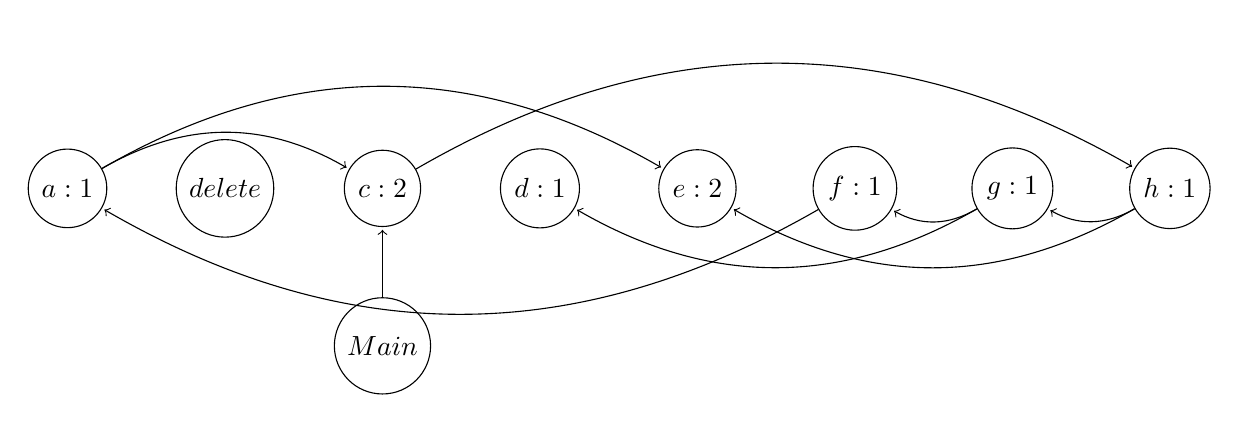
\begin{tikzpicture}[shorten >=1pt,node distance=2cm,on grid,auto]
                      \node[state] 			(a) 					{$a:1$};
                      \node[state] 			(b) 	[right=of a]	{$delete$};
                      \node[state]			(c) 	[right=of b] 	{$c:2$};
                      \node[state] 			(d) 	[right=of c] 	{$d:1$};
                      \node[state] 			(e) 	[right=of d] 	{$e:2$};
                      \node[state] 			(f) 	[right=of e]	{$f:1$};
                      \node[state] 			(g) 	[right=of f]	{$g:1$};
                      \node[state] 			(h) 	[right=of g]	{$h:1$};
                      \node[state] 			(main) 	[below=of c]	{$Main$};
                      \path[->]
                      (a) 	edge	[bend left]		node 	{} 		(e)
                      edge	[bend left] 	node 	{} 		(c)
                      % (b)		edge	[bend left] 	node 	{} 		(d)
                      (c)		edge	[bend left] 	node 	{} 		(h)
                      (f) 	edge	[bend left] 	node 	{} 		(a)
                      (g) 	edge	[bend left] 	node 	{} 		(f)
                      edge	[bend left] 	node 	{} 		(d)
                      (h) 	edge 	[bend left] 	node 	{} 		(e)
                      edge 	[bend left] 	node 	{} 		(g)
                      (main) edge [ ] node {} (c);
                    \end{tikzpicture}\end{center}
                }
          \item (10 pts) Suppose the cost $c_i$ is every reachable words' instruction number, comapare 3 algorithms, let
                $H$ be the size of the heap, let $R$ be the reachable word's data size, when will the Mark and Sweep outperform
                Copy Collector.
                \textcolor{blue}{\\
                  As for memory performance the Mark and Sweep algorithm is O(H), while the Copy Collector algorithm is O(R+H). So the former one outerperforms the latter one when considering the memory cost.\\
                  As for time performance, the former algorithm is $O(R^2+H)$, while the latter one is $O(R^2)$. But when H is not too bigger than R, in which case not too little words are reachable, so that we
                  can omit $O(H)$, and get prettry the same time performance. Still, we have to consider the constant coefficient of both time performance. Mark and Sweep is about $O(2R^2)$, and considering the pseudo code, $c_i=4$. While for Copy Collector, the copy processes comsume plenty of time, comparing
                  to the formal one, despite the have similar $c_i$, the mark and sweep should outerperforms the latter one by constant multiples.
                }
          \item (10 pts) Suppose the marking process is multithreaded, use the above example show that tricolor marking
                with write barrier is thread safe.
                % \textcolor{blue}{\\
                \begin{center}\begin{tikzpicture}[shorten >=1pt,node distance=2cm,on grid,auto]
                    \node[state] 			(a) 					{$a$};
                    \node[state] 			(b) 	[right=of a]	{$b$};
                    \node[state]			(c) 	[right=of b] 	{$c$};
                    \node[state] 			(d) 	[right=of c] 	{$d$};
                    \node[state] 			(e) 	[right=of d] 	{$e$};
                    \node[state] 			(f) 	[right=of e]	{$f$};
                    \node[state] 			(g) 	[right=of f]	{$g$};
                    \node[state] 			(h) 	[right=of g]	{$h$};
                    \node[state] (Main)[below = of c]{$Main$};
                    \path[->]
                    (a) 	edge	[bend left]		node 	{} 		(e)
                    edge	[bend left] 	node 	{} 		(c)
                    (b)		edge	[bend left] 	node 	{} 		(d)
                    (c)		edge	[bend left] 	node 	{} 		(h)
                    (f) 	edge	[bend left] 	node 	{} 		(a)
                    (g) 	edge	[bend left] 	node 	{} 		(f)
                    edge	[bend left] 	node 	{} 		(d)
                    (h) 	edge 	[bend left] 	node 	{} 		(e)
                    edge 	[bend left] 	node 	{} 		(g)
                    (main) edge [ ] node {} (c);
                  \end{tikzpicture}\end{center}


                \begin{center}\begin{tikzpicture}[shorten >=1pt,node distance=2cm,on grid,auto, fill opacity=0.2]
                    \node[state] 			(a) 					{$a$};
                    \node[state] 			(b) 	[right=of a]	{$b$};
                    \node[state, fill=blue]			(c) 	[right=of b] 	{$c$};
                    \node[state] 			(d) 	[right=of c] 	{$d$};
                    \node[state] 			(e) 	[right=of d] 	{$e$};
                    \node[state] 			(f) 	[right=of e]	{$f$};
                    \node[state] 			(g) 	[right=of f]	{$g$};
                    \node[state, fill=red] 			(h) 	[right=of g]	{$h$};
                    \node[state] (Main)[below = of c]{Main};
                    \path[->]
                    (a) 	edge	[bend left]		node 	{} 		(e)
                    edge	[bend left] 	node 	{} 		(c)
                    (b)		edge	[bend left] 	node 	{} 		(d)
                    (c)		edge	[bend left] 	node 	{} 		(h)
                    (f) 	edge	[bend left] 	node 	{} 		(a)
                    (g) 	edge	[bend left] 	node 	{} 		(f)
                    edge	[bend left] 	node 	{} 		(d)
                    (h) 	edge 	[bend left] 	node 	{} 		(e)
                    edge 	[bend left] 	node 	{} 		(g)
                    (main) edge [ ] node {} (c);
                  \end{tikzpicture}\end{center}

                \begin{center}\begin{tikzpicture}[shorten >=1pt,node distance=2cm,on grid,auto, fill opacity=0.2]
                    \node[state] 			(a) 					{$a$};
                    \node[state] 			(b) 	[right=of a]	{$b$};
                    \node[state]			(c) 	[right=of b] 	{$c$};
                    \node[state] 			(d) 	[right=of c] 	{$d$};
                    \node[state,fill=red]		(e) 	[right=of d] 	{$e$};
                    \node[state] 			(f) 	[right=of e]	{$f$};
                    \node[state,fill=red] 			(g) 	[right=of f]	{$g$};
                    \node[state,  fill=blue] 			(h) 	[right=of g]	{$h$};
                    \node[state] (Main)[below = of c]{Main};
                    \path[->]
                    (a) 	edge	[bend left]		node 	{} 		(e)
                    edge	[bend left] 	node 	{} 		(c)
                    (b)		edge	[bend left] 	node 	{} 		(d)
                    (c)		edge	[bend left] 	node 	{} 		(h)
                    (f) 	edge	[bend left] 	node 	{} 		(a)
                    (g) 	edge	[bend left] 	node 	{} 		(f)
                    edge	[bend left] 	node 	{} 		(d)
                    (h) 	edge 	[bend left] 	node 	{} 		(e)
                    edge 	[bend left] 	node 	{} 		(g)
                    (main) edge [ ] node {} (c);
                  \end{tikzpicture}\end{center}

                \begin{center}\begin{tikzpicture}[shorten >=1pt,node distance=2cm,on grid,auto, fill opacity=0.2]
                    \node[state] 			(a) 					{$a$};
                    \node[state] 			(b) 	[right=of a]	{$b$};
                    \node[state]			(c) 	[right=of b] 	{$c$};
                    \node[state,  fill=red]	(d) 	[right=of c] 	{$d$};
                    \node[state, fill=blue]		(e) 	[right=of d] 	{$e$};
                    \node[state,  fill=red] 			(f) 	[right=of e]	{$f$};
                    \node[state, fill=blue] 			(g) 	[right=of f]	{$g$};
                    \node[state ] 			(h) 	[right=of g]	{$h$};
                    \node[state] (Main)[below = of c]{Main};
                    \path[->]
                    (a) 	edge	[bend left]		node 	{} 		(e)
                    edge	[bend left] 	node 	{} 		(c)
                    (b)		edge	[bend left] 	node 	{} 		(d)
                    (c)		edge	[bend left] 	node 	{} 		(h)
                    (f) 	edge	[bend left] 	node 	{} 		(a)
                    (g) 	edge	[bend left] 	node 	{} 		(f)
                    edge	[bend left] 	node 	{} 		(d)
                    (h) 	edge 	[bend left] 	node 	{} 		(e)
                    edge 	[bend left] 	node 	{} 		(g)
                    (main) edge [ ] node {} (c);
                  \end{tikzpicture}\end{center}


                \begin{center}\begin{tikzpicture}[shorten >=1pt,node distance=2cm,on grid,auto, fill opacity=0.2]
                    \node[state,  fill=red] 			(a) 					{$a$};
                    \node[state] 			(b) 	[right=of a]	{$b$};
                    \node[state]			(c) 	[right=of b] 	{$c$};
                    \node[state,  fill=blue]	(d) 	[right=of c] 	{$d$};
                    \node[state]		(e) 	[right=of d] 	{$e$};
                    \node[state,  fill=blue] 			(f) 	[right=of e]	{$f$};
                    \node[state] 			(g) 	[right=of f]	{$g$};
                    \node[state ] 			(h) 	[right=of g]	{$h$};
                    \node[state] (Main)[below = of c]{Main};
                    \path[->]
                    (a) 	edge	[bend left]		node 	{} 		(e)
                    edge	[bend left] 	node 	{} 		(c)
                    (b)		edge	[bend left] 	node 	{} 		(d)
                    (c)		edge	[bend left] 	node 	{} 		(h)
                    (f) 	edge	[bend left] 	node 	{} 		(a)
                    (g) 	edge	[bend left] 	node 	{} 		(f)
                    edge	[bend left] 	node 	{} 		(d)
                    (h) 	edge 	[bend left] 	node 	{} 		(e)
                    edge 	[bend left] 	node 	{} 		(g)
                    (main) edge [ ] node {} (c);
                  \end{tikzpicture}\end{center}
                % }
        \end{enumerate}
\end{enumerate}
\end{document}

